\section{Dodatek}
\subsection{Przyjmowanie Komunii Św. - z instrukcji M. Rumina}
\label{komunia}

\begin{itemize}
  \item na znak \cc1 \aa1 bierze z kredencji obrus komunijny, razem z \aa2
        klękają pośrodku, wchodzą na najwyższy stopień ołtarza i klękają
        twarzami do siebie (jeszcze nie rozkładają obrusu)
  \item ministranci biorący udział w lucenarium wchodzą dwójkami do
        prezbiterium, tworząc w ten sposób naturalną „kolejkę” do Komunii św.
        Przed nimi do kolejki wchodzą księża, klerycy  \footnote{W Wielki Piątek
        najprawdopodobniej nie będzie żadny kleryków ani księży. W takim razie
        wzmianki o nich pomijamy, a na rysunkach w ich miejsce wstawiamy pustą
        przestrzeń} i \cc1, za nimi reszta ministrantów z chóru. \cc1 – zależnie
        od ilości duchownych i ministrantów może staje do komunii sam lub w
        parze
  \item po \textit{Indulgentiam} rozkładany jest obrus komunijny

        \begin{figure}[h]
          \centering
          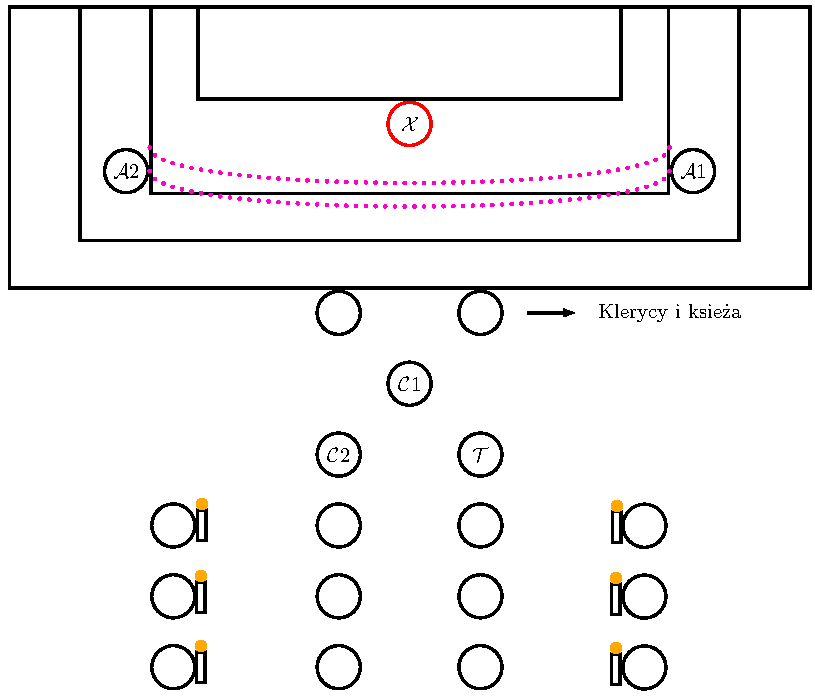
\includegraphics[scale=0.5]{Piatek/Komunia1.pdf}
        \end{figure}

  \item \cc1 podaje patenę pierwszemu duchownemu przyjmującemu Komunię św., albo
        jeśli nie ma duchownych trzyma ją sam. Po przyjęciu Komunii Św. zajmuje
        miejsce przy \ii~, gdzie asystuje z pateną
  \item \cc2 lub \tt~ po przyjęciu Komunii św. zajmuje miejsce przy celebransie
        ze świeczką sanctusową

        \begin{figure}[h]
          \centering
          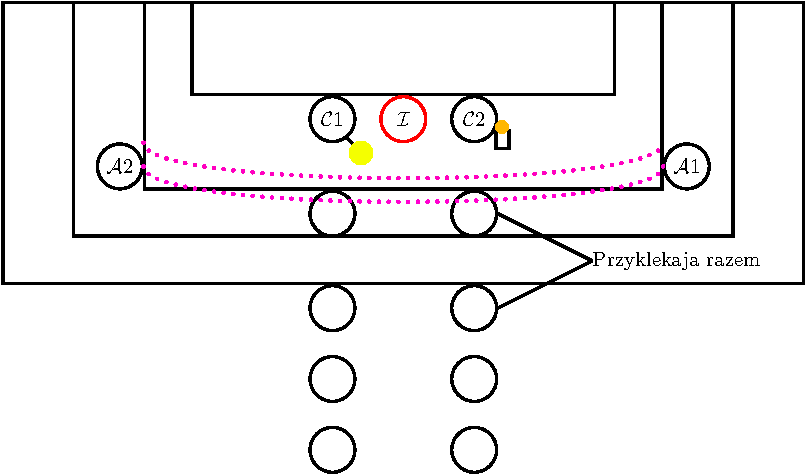
\includegraphics[scale=0.5]{Piatek/Komunia2.pdf}
        \end{figure}

  \item \aa1 i \aa2 trzymający obrus przyjmują Komunię św. razem z \cc1
  \item każda dwójka przystępująca do Komunii św. przyklęka \textbf{jednocześnie
          z poprzedzającą parą}, wchodzi na stopnie i klęka na dwa kolana. Po
          przyjęciu komunii znów przyklęka jednocześnie z parą stojącą za nimi.
          Ze stopni ołtarza schodzimy w lewo – do chóru.
  \item po przyjęciu Komunii Św. przez ministrantów \aa1 i \aa2 wstają i
        przechodzą do miejsca udzielalnia komunii wiernym. Z pateną i świeczką
        sanctusową asystują \cc1 i \cc2

        \begin{figure}[h]
          \centering
          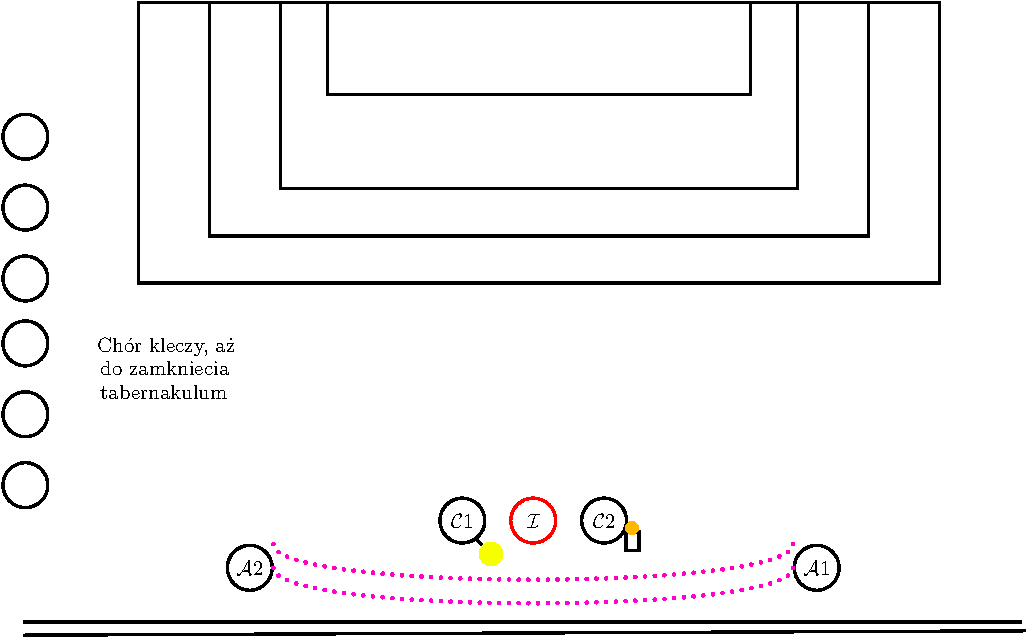
\includegraphics[scale=0.5]{Piatek/Komunia3.pdf}
        \end{figure}

\end{itemize}

\newpage

\section{Do poprawy}
\begin{itemize}
  \item Sprawdizć wcześniej czy są poprawne modlitwy na Żydów w OHS-ie
  \item Wybrać kompetentnych ministarntów do pateny i świeczki sanktusowej lub
        niech robią to ceremoniarze
\end{itemize}